\appendix

\chapter{HDL Railroad Diagrams}
\label{appendix:hdl-railroad}

\noindent
\includesvg{HDL_Railroad_1}

\vspace{20pt}

\noindent
\includesvg{HDL_Railroad_2a}

\noindent
\includesvg{HDL_Railroad_2b}

\vspace{20pt}

\noindent
\includesvg{HDL_Railroad_3}

\vspace{20pt}

\noindent
\includesvg[width=380pt]{HDL_Railroad_4}

\vspace{20pt}

\noindent
\includesvg{HDL_Railroad_5a}

\noindent
\includesvg{HDL_Railroad_5b}

\vspace{20pt}

\noindent
\includesvg[width=380pt]{HDL_Railroad_6}

\vspace{20pt}

\noindent
\includesvg{HDL_Railroad_7}

\vspace{20pt}

\noindent
\includesvg{HDL_Railroad_8}

\chapter{HDL Token, Grammar Definition}
\label{appendix:hdl-grammar}

This appendix is also available online with syntax highlighting \& easier to browse at \href{https://github.com/durasj/chipsandcode/blob/6decf05115ba1d4ca927de42f63c8431b1ac3124/src/lib/editor/hdl/grammar.ne}{github.com/durasj/chipsandcodeblob/6decf05/src/lib/editor/hdl}.

\inputminted[breaklines=true,fontsize=\footnotesize]{text}{./assets/hdl.ne}

\chapter{HDL Example}
\label{appendix:hdl-example}

\inputminted[breaklines=true,fontsize=\footnotesize]{text}{./assets/Xor.hdl}

\chapter{TST Railroad Diagrams}
\label{appendix:tst-railroad}

\noindent
\includesvg{TST_Railroad_1}

\vspace{20pt}

\noindent
\includesvg[width=380pt]{TST_Railroad_2}

\vspace{20pt}

\noindent
\includesvg{TST_Railroad_3}

\vspace{20pt}

\noindent
\includesvg{TST_Railroad_4}

\vspace{20pt}

\noindent
\includesvg{TST_Railroad_5}

\vspace{20pt}

\noindent
\includesvg[width=380pt]{TST_Railroad_6}

\vspace{20pt}

\noindent
\includesvg{TST_Railroad_7}

\vspace{20pt}

\noindent
\includesvg{TST_Railroad_8}

\chapter{TST Token, Grammar Definition}
\label{appendix:tst-grammar}

This appendix is also available online with syntax highlighting \& easier to browse at \href{https://github.com/durasj/chipsandcode/blob/6decf05115ba1d4ca927de42f63c8431b1ac3124/src/lib/editor/tst/grammar.ne}{github.com/durasj/chipsandcodeblob/6decf05/src/lib/editor/tst}.

\inputminted[breaklines=true,fontsize=\footnotesize]{text}{./assets/tst.ne}

\chapter{TST Example}
\label{appendix:tst-example}

\inputminted[breaklines=true,fontsize=\footnotesize]{text}{./assets/Xor.tst}

\chapter{WCAG Evaluation Report}
\label{appendix:wcag-report}

Below is the \gls{wcag} evaluation report generated using the \gls{wcagem} report tool.

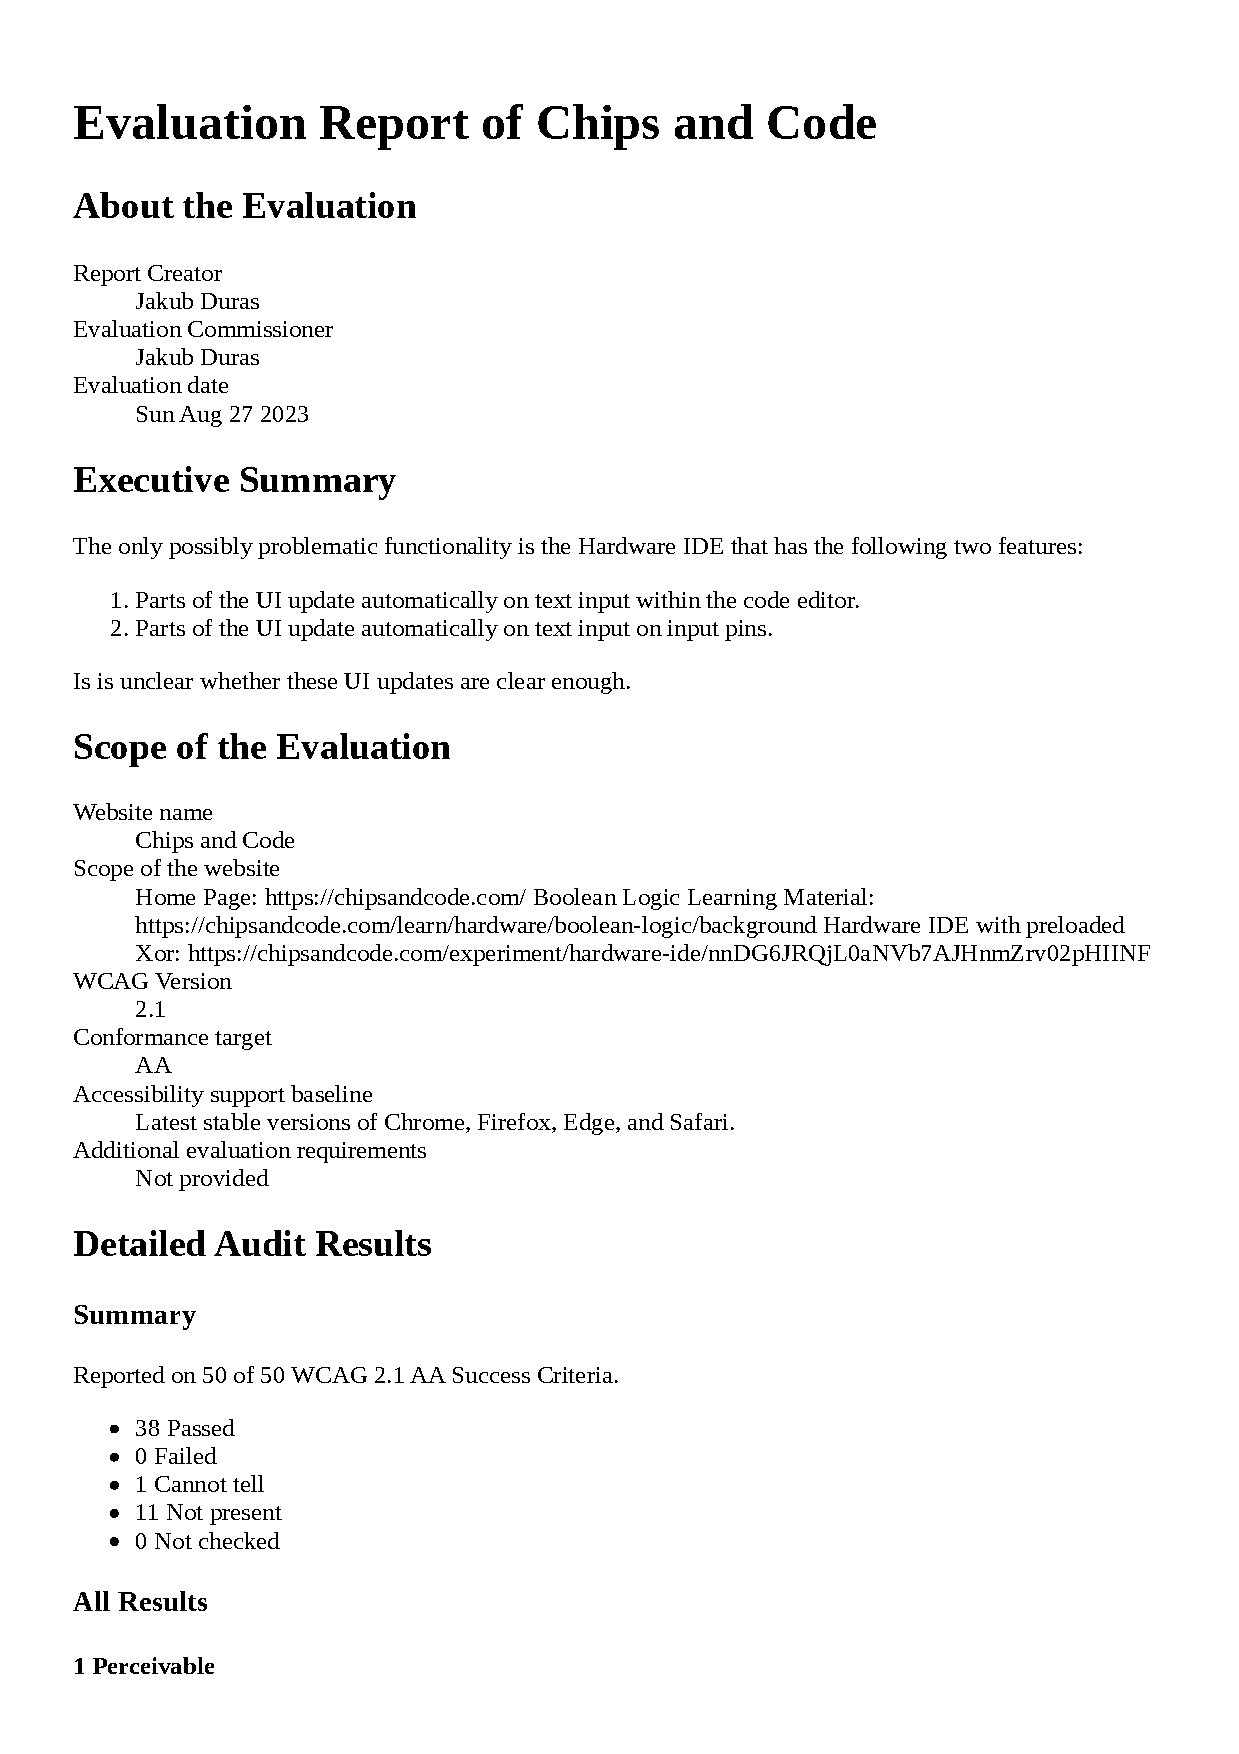
\includepdf[pages=-, pagecommand={}, width=\textwidth]{WCAG_Evaluation_Report.pdf}

\chapter{Study Time Data}
\label{appendix:study-time-notes}

Below are raw timestamp data and notes collected during and after the study session for each participant.
This appendix is also alternatively available online as a \href{https://docs.google.com/spreadsheets/d/1CGNs1pCKvGJ4QuRDCExNc_3SZ4pgX3UlTXSKJU8hpa8}{Google Spreadsheet}.

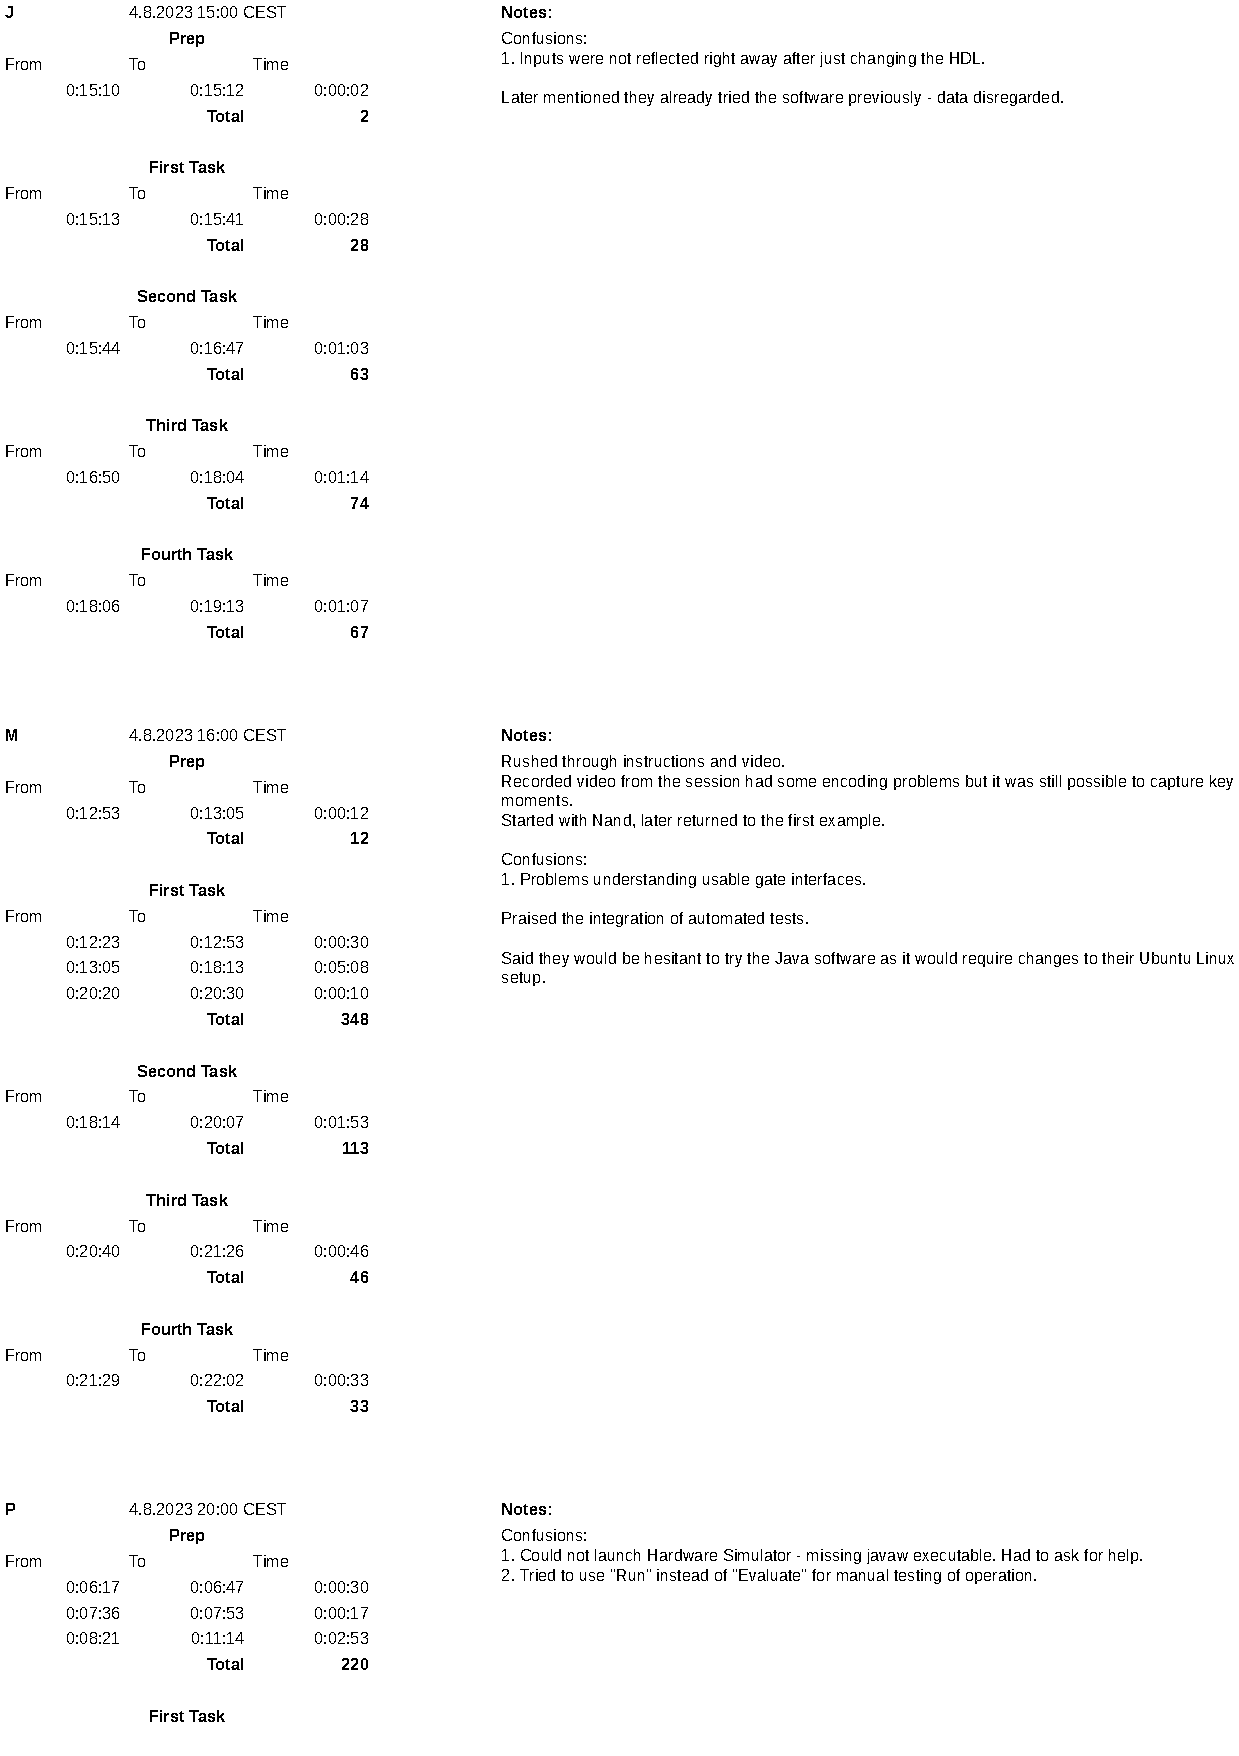
\includepdf[pages=-, pagecommand={}, width=\textwidth]{Study_Raw_Data.pdf}

\chapter{Study SUS Scores}
\label{appendix:study-sus}

The data presented in this appendix are also alternatively available online within a \href{https://docs.google.com/spreadsheets/d/1CGNs1pCKvGJ4QuRDCExNc_3SZ4pgX3UlTXSKJU8hpa8}{Google Spreadsheet}.

\section*{Group A}

\begin{tabular}{llllllllllll}
    \rotheading[50][1.5em]{Person} & \rotheading[50][1.5em]{1. Frequently} & \rotheading[50][1.5em]{2. Complex} & \rotheading[50][1.5em]{3. Easy to Use} & \rotheading[50][1.5em]{4. Technical support} & \rotheading[50][1.5em]{5. Well Integrated} & \rotheading[50][1.5em]{6. Inconsistency} & \rotheading[50][1.5em]{7. Learn Quickly} & \rotheading[50][1.5em]{8. Awkward} & \rotheading[50][1.5em]{9. Felt Confident} & \rotheading[50][1.5em]{10. Learn Lot} & \rotheading[50][1.5em]{Score} \\ \hline
    \textbf{M} & 4 & 2 & 5 & 3 & 5 & 2 & 5 & 2 & 3 & 2 & 77.5 \\ 
    \textbf{LU} & 5 & 1 & 5 & 4 & 5 & 1 & 3 & 1 & 5 & 2 & 85 \\ 
    \textbf{Y} & 5 & 1 & 5 & 2 & 5 & 1 & 5 & 1 & 5 & 3 & 92.5 \\ 
    \textbf{MI} & 3 & 1 & 5 & 1 & 4 & 2 & 5 & 1 & 4 & 2 & 85 \\ 
    \textbf{MX} & 1 & 1 & 5 & 1 & 5 & 1 & 3 & 2 & 5 & 1 & 82.5 \\ 
    \textbf{R} & 4 & 1 & 5 & 1 & 4 & 1 & 3 & 1 & 4 & 1 & 87.5 \\ 
    \textbf{MK} & 5 & 1 & 5 & 1 & 5 & 1 & 4 & 1 & 5 & 1 & 97.5 \\ 
    \textbf{L} & 5 & 1 & 5 & 1 & 5 & 1 & 5 & 1 & 5 & 1 & 100 \\ 
    \textbf{MA} & 4 & 3 & 4 & 4 & 4 & 2 & 4 & 2 & 3 & 2 & 65 \\ 
    \textbf{KY} & 5 & 1 & 5 & 2 & 4 & 1 & 5 & 1 & 5 & 1 & 95 \\ 
    \textbf{KA} & 4 & 2 & 5 & 2 & 4 & 2 & 5 & 2 & 4 & 3 & 77.5 \\ 
    \textbf{E} & 4 & 1 & 5 & 1 & 5 & 1 & 4 & 1 & 5 & 1 & 95
\end{tabular}

\section*{Group B}

\begin{tabular}{llllllllllll}
    \rotheading[50][1.5em]{Person} & \rotheading[50][1.5em]{1. Frequently} & \rotheading[50][1.5em]{2. Complex} & \rotheading[50][1.5em]{3. Easy to Use} & \rotheading[50][1.5em]{4. Technical support} & \rotheading[50][1.5em]{5. Well Integrated} & \rotheading[50][1.5em]{6. Inconsistency} & \rotheading[50][1.5em]{7. Learn Quickly} & \rotheading[50][1.5em]{8. Awkward} & \rotheading[50][1.5em]{9. Felt Confident} & \rotheading[50][1.5em]{10. Learn Lot} & \rotheading[50][1.5em]{Score} \\ \hline
    \textbf{P} & 3 & 2 & 4 & 2 & 4 & 1 & 5 & 2 & 5 & 1 & 82.5 \\
    \textbf{S} & 3 & 2 & 4 & 3 & 4 & 3 & 5 & 2 & 4 & 2 & 70 \\ 
    \textbf{MM} & 4 & 2 & 4 & 1 & 5 & 1 & 5 & 2 & 5 & 1 & 90 \\ 
    \textbf{SA} & 3 & 4 & 2 & 2 & 2 & 4 & 3 & 4 & 2 & 3 & 37.5 \\ 
    \textbf{JO} & 4 & 1 & 3 & 3 & 5 & 1 & 4 & 1 & 3 & 2 & 77.5 \\ 
    \textbf{PE} & 3 & 1 & 4 & 1 & 5 & 1 & 5 & 1 & 5 & 1 & 92.5 \\ 
    \textbf{MS} & 5 & 2 & 5 & 1 & 5 & 1 & 5 & 1 & 5 & 1 & 97.5 \\ 
    \textbf{B} & 4 & 1 & 5 & 1 & 4 & 1 & 5 & 3 & 5 & 2 & 87.5 \\ 
    \textbf{V} & 4 & 4 & 4 & 2 & 2 & 1 & 4 & 4 & 5 & 2 & 65 \\ 
    \textbf{MH} & 5 & 2 & 4 & 1 & 4 & 1 & 5 & 1 & 4 & 1 & 90 \\ 
    \textbf{LB} & 4 & 2 & 4 & 2 & 4 & 1 & 3 & 1 & 4 & 3 & 75 \\ 
    \textbf{MT} & 4 & 2 & 4 & 1 & 5 & 1 & 5 & 1 & 5 & 2 & 90
\end{tabular}
